
\section{动态规划基础------序列型DP}
序列型dp是动态规划中一个常见的模型.
\subsection{最长上升子序列问题---LIS}
\subsubsection{介绍与实现}
\begin{definition}[最长上升子序列]
	给出一个序列$a_1, a_2, \cdots, a_n$,求它的一个子序列(设为$s_1, s_2, \cdots, s_n$),使得这个子序列满足这样的性质:$s_1<s_2<s_3<\cdots<s_n$并且这个子序列的长度最长。输出这个最长的长度。
\end{definition}

以上是最长上升子序列的定义。


考虑状态dp[i]表示当前枚举到了第i个数,当前最长上升子序列长度为dp[i]。

用$arr$表示原序列,$dp$表示最长上升子序列的长度。我们枚举每一个序列中的每一个元素$i$,并且枚举$i$前面所有的数$j$。如果$i>j$,那么最长上升子序列的长度一定至少比$dp(j)$大1(为什么?).
状态转移方程为:
\begin{equation*}
dp(i)=\max_{j<i,arr_i>arr_j}\{dp(j)+1\}
\end{equation*}
\begin{minted}{C++}
dp[1] = 1;  
for(int i = 2; i <= n; ++i)  
{
    for(int j = 1; j < i; ++j)
        if(arr[i] > arr[j])  
            dp[i] = max(dp[i], dp[j]+1);  
}
\end{minted}

时间复杂度$O(n^2)$。

当然这不是最优的方法,考虑一下如何优化?

显然第二层枚举不是必需的。第二层枚举的作用是找到最接近且比当前枚举的数。所以可以使用二分查找优化掉这一层循环。

我们考虑某一个元素对之后最长上升子序列有贡献的话仅当后面存在比它元素更大的值, 也就是说最长上升子序列中的元素越小越好. 也就是说如果两个长度相同的最长上升子序列但是最后元素大小不同,肯定是最后元素越小的元素对答案的贡献大.

增加一个$b$,$b(i)$用以表示长度为$i$最长上升子序列的最后元素的大小,$k$表示$b$的长度,所以如果当前元素大于当前最长子序列的最后元素的话, 说明当前元素可以使当前最长上升子序列长度增加 1 .如果当前元素可以替换掉之前某一上升子序列的最后元素使得
则:

\begin{equation*}
	dp[i]=\begin{cases}
		b[k+1]=arr[i]                  & , arr[i]>b[k] \\
		b[binary\_search(arr[i],1,k)] & , arr[i]<b[k]
	\end{cases}
\end{equation*}

容易发现,b数组始终是单调递增的。所以我们可以二分查找arr[i]在b数组出现的位置,从而把时间复杂度降至$O(n\log n)$。

二分应该都会吧?如果不会二分的话就看看代码:

\begin{minted}{C++}
int binarySearch(const int *Array,int start,int end,int key)
//Array:待查找的数组,start:起始点下标,end:终止点下标,key:待查找的数。
{
    int left,right;
    int mid;
    left=start;
    right=end;
    while(left<=right)
    {
        mid=(left+right)/2;
        if(key==Array[mid])  return mid;
        else if(key<Array[mid]) right=mid-1;
        else if(key>Array[mid]) left=mid+1;    
     }
     return -1;//没有找到
}
\end{minted}

以上二分代码适用于一般情况,更常用的写法:
\begin{minted}{C++}
int binarySearch(int num, int l, int r)
//num为待查找的数。
{    
    while(l <= r)    
    {    
        int mid = (l+r)/2;    
        if(num >= b[mid])    
            l = mid + 1;    
        else  
            r = mid - 1;    
    }    
    return l;
}
\end{minted}

当然如果愿意用STL的话,lower\_bound()函数也很好用:

\begin{minted}{C++}
#include<algorithm>
std::lower_bound(first,last,val);//在区间[first,last)中二分查找元素val。
//如果找到相应的val,则返回一个指向元素位置的指针;
//否则返回一个指向最接近val且小于val的元素位置的指针。
//另外一种用法:
std::lower_bound(first,last,val,comp);
//以自定义comp作为比较器进行比较(类似sort的用法),返回值同上。
//同理还有upper_bound()函数。
\end{minted}
\subsubsection{LIS的打印}
在状态转移的时候记录一波转移方向,保存在pre[]数组中,然后需要输出的时候就可以根据pre[]数组逆序构造出LIS,使用一个栈保存起来就可以正向输出了。

代码实现起来比较容易,自己写一下,也不那么常用。
\subsubsection{例题---导弹拦截}
\begin{example}导弹拦截\\
	\textbf{题目描述}

	某国为了防御敌国的导弹袭击,发展出一种导弹拦截系统。但是这种导弹拦截系统有一个缺陷:虽然它的第一发炮弹能够到达任意的高度,但是以后每一发炮弹都不能高于前一发的高度。某天,雷达捕捉到敌国的导弹来袭。由于该系统还在试用阶段,所以只有一套系统,因此有可能不能拦截所有的导弹。

	输入导弹依次飞来的高度(雷达给出的高度数据是不大于50000的正整数),计算这套系统最多能拦截多少导弹,如果要拦截所有导弹最少要配备多少套这种导弹拦截系统。\\
	\textbf{输入输出格式}
	\ \\
	\textbf{输入格式:}

	一行,若干个整数(个数少于100000)
	\ \\
	\textbf{输出格式:}

	2行,每行一个整数,第一个数字表示这套系统最多能拦截多少导弹,第二个数字表示如果要拦截所有导弹最少要配备多少套这种导弹拦截系统。
	\ \\
	\textbf{输入输出样例}
	\ \\
	\textbf{输入样例:}
	\begin{minted}{text}
389 207 155 300 299 170 158 65
\end{minted}
	\textbf{输出样例:}
	\begin{minted}{text}
6
2
\end{minted}
\end{example}

导弹拦截这道题目出自NOIp 1999,容易看出是一个LIS问题(最长不升子序列是LIS的一个变形)。可以直接使用LIS看看能不能拿到满分。


\note
\subsection{最长公共子序列---LCS}
\subsubsection{介绍与实现}
\begin{definition}[最长公共子序列]
一个数列,如果分别是两个或多个已知数列的子序列,且是所有符合此条件序列中最长的,则称为已知序列的最长公共子序列。在计算机科学中,最长递增子序列是指,在一个给定的数值序列中,找到一个子序列,使得这个子序列元素的数值依次递增,并且这个子序列的长度尽可能地大。
\end{definition}

以上是对最长公共子序列问题的定义。理解一下。

考虑一下这种题目如何打暴力。

非常容易,对吧,就是暴力枚举第一个序列的每一个子序列,对每一个子序列判断它是否为第二个序列的子序列。然而这样的时间复杂度是$O(2^{\min(n,m)})$的,其中n, m为字符串的长度。

思考这样一个性质:如果一个LCS是另一个LCS的前缀,那么一定存在一个LCS,使得它的长度为这两个LCS长度之和。

\begin{thm}[LCS的最优子结构]
	令$X=\langle x_1, x_2, \cdots, x_m\rangle$和$Y=\langle y_1, y_2,$ $\cdots,y_n\rangle$为两个序列,$Z=\langle z_1, z_2, \cdots, z_k\rangle$为X和Y的任意LCS。
	\begin{enumerate}
		\item{如果$x_m=y_n$,则$z_k=x_m=y_n$。且$Z_{k-1}$是$X_{m-1}$和$Y_{n-1}$的一个LCS。}
		\item{如果$x_m\neq y_n$,那么$x_m\neq y_n$意味着$Z$是$X_{m-1}$和$Y$的一个LCS。}
		\item{如果$x_m\neq y_n$,那么$z_k\neq y_n$意味着$Z$是$X$和$Y_{n-1}$的一个LCS。}
	\end{enumerate}
\end{thm}

举个例子:
\begin{center}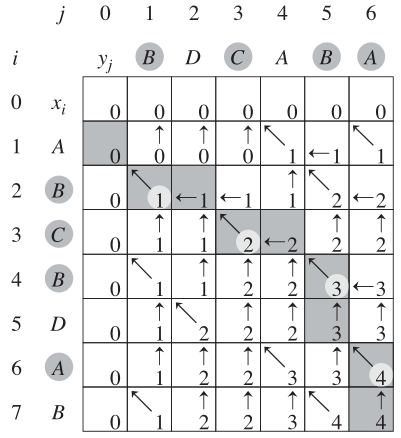
\includegraphics[height=5cm]{CLRS_LCS.png}\end{center}

上图是求$X=\langle A, B, C, D, B, D, A, B\rangle$和$B=\langle B, D, C, A, B, A\rangle$的LCS的过程。

\begin{Proof}
	(1)如果$z_k\neq x_m$,那么可以将$x_m=y_n$追加到$Z$的末尾,得到$X$和$Y$的一个长度为$k+1$的公共子序列。与$Z$是$X$和$Y$的最长公共子序列的假设矛盾。因此,必然有$z_k=x_m=y_n$。这样,前缀$Z_{k-1}$是$X_{m-1}$和$T_{n-1}$的一个长度为$k-1$的公共子序列。我们希望证明它是一个LCS。利用反证法,假设存在$X_{m-1}$和$Y_{n-1}$的一个长度大于$k-1$的公共子序列$W$,则将$x_m=y_n$追加到$W$的末尾会得到$X$和$Y$的一个长度大于$k$的公共子序列,矛盾。

	(2)如果$z_k\neq x_m$,那么$Z$是$X_{m-1}$和$Y$的一个公共子序列。如果存在$X_{m-1}$和Y的一个长度大于$k$的公共子序列$W$,那么$W$也是$X_m$和$Y$的公共子序列,与$Z$是$X$和$Y$的最长公共子序列的假设矛盾。

	(3)与情况(2)对称。\ 
\end{Proof}

于是我们get到了LCS的一个很重要的性质,没有后效性,具有最优子结构的性质。这是LCS问题可以DP的基础。

很容易看出,最初我们写的暴力求解算法中,有大量重叠的子问题(考虑求子序列$X = \langle x_a, x_{a+1}, \cdots, x_b\rangle$的LCS,必定求这个子序列的子序列$Y = \langle x_{a+m}, x_{a+m+1}, \cdots, x_{a+n}\rangle$这个子序列的LCS),所以LCS问题也有重叠子问题性质。

由上述定理我们就可以写出一个递归解。刚才的暴力中我们是枚举每一个子序列,然后进行判断,现在我们考虑能否直接构造出这样的一个序列。

明显的,状态转移有以下两种:
\begin{itemize}
	\item{如果两位相等,那么新的LCS可以连接到旧的LCS之后,构成一个新的较长的LCS。}
	\item{如果两位不相等,那么新的LCS不变,还是前一位的最长的LCS。}
\end{itemize}
设状态f[i][j]表示到字符串X的第i位与字符串Y的第j位的LCS长度,则:
\begin{equation*}
	f[i][j]=\begin{cases}
		f[i-1][j-1]+1             & , X[i]=Y[j]     \\
		\max(f[i][j-1],f[i-1][j]) & , X[i]\neq Y[j].
	\end{cases}
\end{equation*}

根据上面的状态转移方程写出代码即可,时间复杂度$O(nm)$.
\subsubsection{LCS的打印}
同LIS的打印,记录一下转移的方向,然后就可以了,时间复杂度为$O(nm)$。
\subsubsection{LCS的优化}
考虑一下是不是有什么地方还可以优化。

考虑上一节说的LCS的打印的过程,也可以不记录下转移的方向,因为每个状态转移的方向都是固定的,所以可以在$O(1)$的时间内判断出一个状态是由三个状态中的哪一个转移而来的,因此不再需要pre[]数组,只需要在输出过程中逆序转移,判断一下转移方向,把每一个数丢到栈里,再依次输出即可。

对于不需要输出LCS的问题,还可以使用滚动数组优化一下f数组的空间占用。因为每次转移只用到了f数组当前的一行以及前一行,所以只需要保留这两行数据即可。但是如果需要计算LCS的元素,就不能使用滚动数组优化(思考一下为什么)。

例题的话,可以参考一下洛谷P1439 的前50\%,至于后面的优化,建议参考一下题解,因为严格意义上这个优化意义不是很大,常数也很大,不是那么实用。

\note

\newpage\